\documentclass{article}

\usepackage{fullpage}  % Makes the text margins smaller
\usepackage{graphicx} % To include figures
\usepackage{fancyvrb} % Includes the \VerbatimInput command to read in code files
\usepackage{amsmath}
\DeclareGraphicsExtensions{.png}
\renewcommand*{\arraystretch}{2}

\author{Cody Lieu, Yixin Lin}
\title{COMPSCI 527 Homework 5}

\begin{document}
\maketitle

\section*{Problem 1(a)}

Points tracked well: 1, 3, 4, 5

Points lost during tracking: 2

Points tracked but don't correspond to fixed points in the world: 6

Point 2 was lost during tracking, which is clearly not satisfactory because during reconstruction, that 3-d information that corresponds to that point is lost and cannot be used to generate the point cloud.

Point 6 was tracked but don't correspond to a fixed point in the world, which would be problematic in reconstruction because the point would be constructed using incorrect information, and the resulting point in the point cloud would not represent an actual fixed point in the real world.

\section*{Problem 1(b)}

The last frame in which all features are present is frame 5.

\begin{center}
\begin{tabular}{ ||c|c|c|| } 
	\hline
	Feature & cond(H) & $\sigma_min(H)$ \\ \hline
 	1 &3.19 &49.82 \\ 
	2 &7.14 &0.14 \\
	3 &5.06 &55.04 \\
	4 &7.54 &41.91 \\
	5 &3.45 &161.35 \\
	6 &10.88 &11.20 \\
\hline
\end{tabular}
\end{center}

\section*{Problem 1(c)}
The $\sigma_{min}(H)$ of feature 2 is very close to 0. This means that even if the condition number is ``reasonable'', i.e. not very large, it doesn't matter; this is still a degenerate case of the matrix (the matrix is close to being rank-deficient), which corresponds to an occurence of the aperture problem.

\section*{Problem 1(d)}


\begin{center}
\begin{tabular}{ ||c||c|c|c|| } 
	\hline
				& Newton & gradient descent & grid \\ \hline
	ssd evals 	& 169 & 837 & 5124\\

\hline
\end{tabular}
\end{center}

\section*{Problem 1(e)}

In general, the grid method did worse than the others (off by at least a little bit), while Newton's method and gradient descent worked fairly well. However, Newton's method did fail for a point.

If resolution of the grid was closer to the resolution of the image (the pitch was smaller), then the grid method would have been more effective (but also more costly).

For point 1, all three methods tracked it fairly well (thought the grid method was off by a bit more).

For point 2, interestingly the Newton method failed to track it while the gradient descent method did well. Also, the grid method did not fail to track it but the results are clearly incorrect.

For point 3 and 5, it was tracked well by all three methods (though the grid method was again off by more than the other two).

For point 4, it was tracked well by all three methods.

For point 6, it was tracked by all three similarly (grid method was again off by more than the other two) but did not correspond to a fixed point in space.


\section*{Problem 1(f)}

The camera moved forward, since the tracking points look like they got closer (the image got slightly larger, and the points ``expanded'').

\section*{Problem 2(a)}

\begin{center}
Gradient:
\[
	\begin{bmatrix}
		-2a + 4bx_1^3 -4bx_1x_2 + 2x_1\\ 
		2b(x_2-x_1^2)
	\end{bmatrix}
\]

Hessian:
\[
	\begin{bmatrix}
		12bx_1^2-4bx_2+2 & -4bx_1\\
		-4bx_1 & 2b 
	\end{bmatrix}
\]
\end{center}

\section*{Problem 2(b)}


$\mathbf{x^{*}} = $
\[
	\begin{bmatrix}
		a \\
		a^2
	\end{bmatrix}
\]

$f(\mathbf{x^{*}}) = 0$
	

\section*{Problem 2(c)}

\VerbatimInput[fontsize=\small,fontshape=n,xleftmargin=15mm]{code/bananaCost.m}

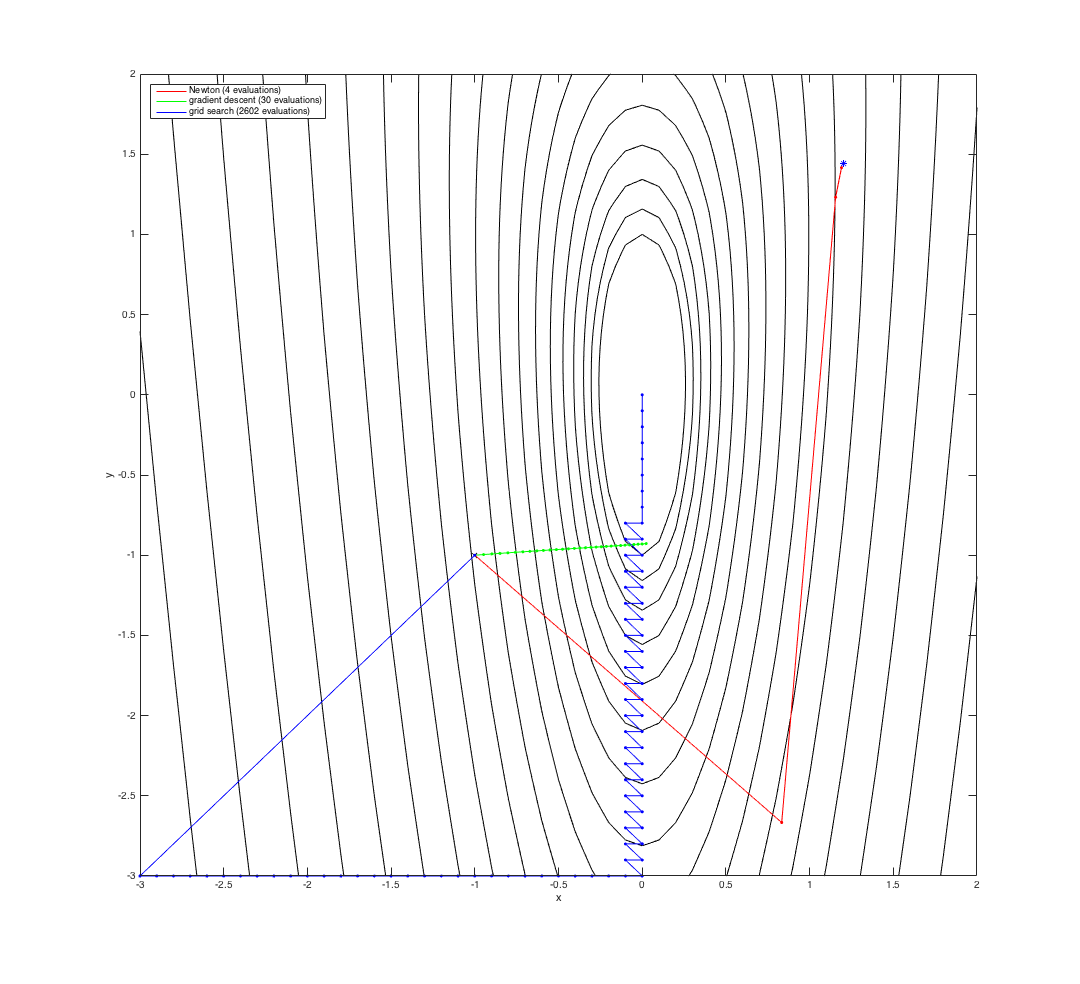
\includegraphics[scale=0.5]{code/2c.png}

\section*{Problem 2(d)}

The grid search method failed to converge in the maximum number of iterations allowed; it converged in 2602 iterations.

\section*{Problem 2(e)}

Newton's method took the fewest iterations (9 iterations).

\section*{Problem 2(f)}

No, individual iterations for Newton's method are the most expensive, and the iterations for the grid method are the least expensive.

\section*{Problem 2(g)}

The grid method goes through every point in the grid it lays out (the density of which depends on the pitch), and finds the minimum point within those. It updates a new minimum every time it finds a new point that's smaller than the previous minimum. This means that the path that the grid method travels are the ``current minimums'', which makes perfect sense since it traverses from [-2, -2] to [3, 3] at a pitch of 0.1, trying x values before y values. 

Thus, the points look like they're going down the gradient, because it only updates the current minimum when it finds a smaller minimum. Also, it looks like it travels straight line segments, since the only points it considers are those that lie on the grid it lays out. Finally, it goes right and then up, since that's the order in which it considers the points (points with ascending x values for each ascending y value).

\section*{Problem 2(h)}

For grid search to achieve a similar accuracy to Newton's method, it needs to have a finer grid (i.e. a smaller pitch). Since the actual minimum is [1,2, 1.44], the pitch needs to be 0.01 instead of 0.1. By decreasing the pitch by a factor of 10, we increase the costliness by a factor of 100. This depends on the dimension: decreasing the pitch by a factor of $p$ increases the costliness by a factor of $p^n$ where $n$ is the number of dimensions.

\end{document}